\documentclass{article}
\usepackage{tikz}

\begin{document}

\begin{figure}[h]
    \centering
    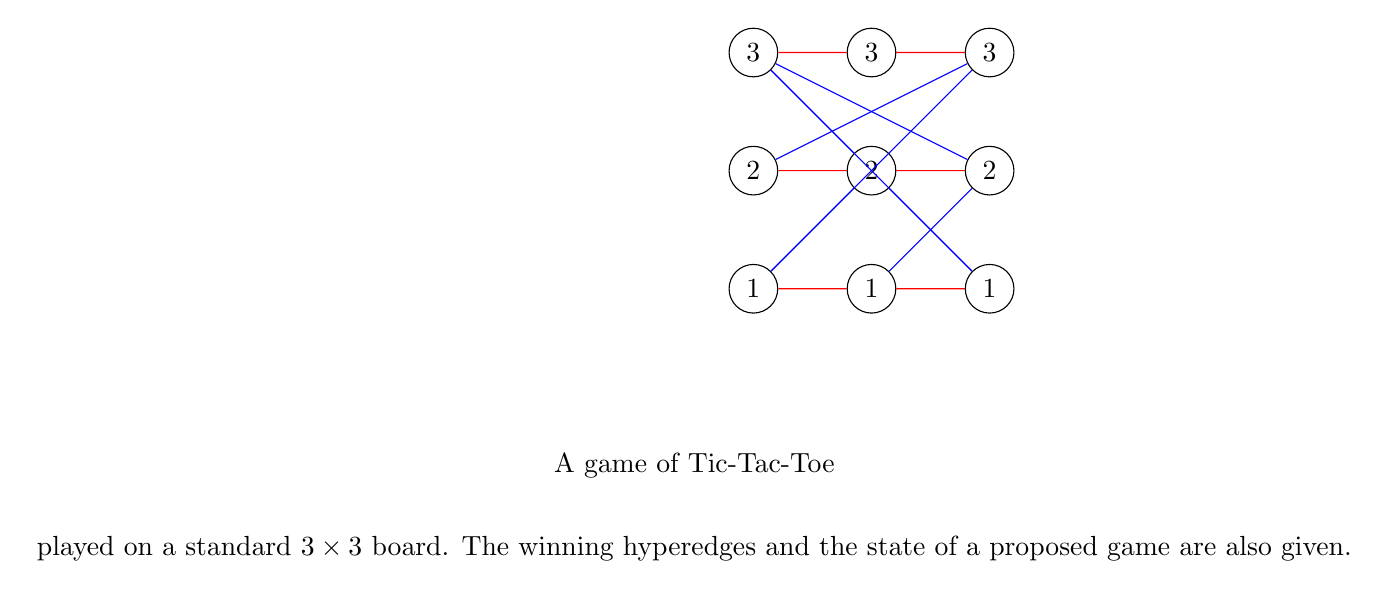
\begin{tikzpicture}[scale=1.5]
        % Define nodes
        \foreach \x in {1,...,3} {
            \foreach \y in {1,...,3} {
                \node[circle, draw, fill=white] (n\x\y) at (\x,\y) {\y};
            }
        }
        
        % Draw edges
        \draw[red] (n11) -- (n21);
        \draw[red] (n21) -- (n31);
        \draw[red] (n12) -- (n22);
        \draw[red] (n22) -- (n32);
        \draw[red] (n13) -- (n23);
        \draw[red] (n23) -- (n33);
        
        \draw[blue] (n11) -- (n22);
        \draw[blue] (n11) -- (n33);
        \draw[blue] (n21) -- (n32);
        \draw[blue] (n31) -- (n22);
        \draw[blue] (n31) -- (n13);
        \draw[blue] (n12) -- (n33);
        \draw[blue] (n22) -- (n13);
        \draw[blue] (n32) -- (n13);
        
        % Add labels
        \node at (0.5,-0.5) {A game of Tic-Tac-Toe};
        \node at (0.5,-1.2) {played on a standard $3 \times 3$ board. The winning hyperedges and the state of a proposed game are also given.};
    \end{tikzpicture}
\end{figure}

\end{document}